
%package list
\documentclass{article}
\usepackage{amsmath}
\usepackage[top=3cm, bottom=3cm, outer=3cm, inner=3cm]{geometry}
\usepackage{multicol}
\usepackage{graphicx}
\usepackage{url}
%\usepackage{cite}
\usepackage{hyperref}
\usepackage{array}
%\usepackage{multicol}
\newcolumntype{x}[1]{>{\centering\arraybackslash\hspace{0pt}}p{#1}}
\usepackage{natbib}
\usepackage{pdfpages}
\usepackage{multirow}
\usepackage[normalem]{ulem}
\useunder{\uline}{\ul}{}
\usepackage{svg}
\usepackage{xcolor}
\usepackage{listings}
\lstdefinestyle{ascii-tree}{
    literate={├}{|}1 {─}{--}1 {└}{+}1 
  }
\lstset{basicstyle=\ttfamily,
  showstringspaces=false,
  commentstyle=\color{red},
  keywordstyle=\color{blue}
}
%\usepackage{booktabs}
\usepackage{caption}
\usepackage{subcaption}
\usepackage{float}
\usepackage{array}

\newcolumntype{M}[1]{>{\centering\arraybackslash}m{#1}}
\newcolumntype{N}{@{}m{0pt}@{}}


%%%%%%%%%%%%%%%%%%%%%%%%%%%%%%%%%%%%%%%%%%%%%%%%%%%%%%%%%%%%%%%%%%%%%%%%%%%%
%%%%%%%%%%%%%%%%%%%%%%%%%%%%%%%%%%%%%%%%%%%%%%%%%%%%%%%%%%%%%%%%%%%%%%%%%%%%
\newcommand{\itemEmail}{ccapatinta@unsa.edu.pe}
\newcommand{\itemStudent}{Capatinta Almanza Camilo B. A.}
\newcommand{\itemCourse}{Lab. Análisis y Diseño de Algoritmos}
\newcommand{\itemCourseCode}{1702231}
\newcommand{\itemSemester}{IV}
\newcommand{\itemUniversity}{Universidad Nacional de San Agustín de Arequipa}
\newcommand{\itemFaculty}{Facultad de Ingeniería de Producción y Servicios}
\newcommand{\itemDepartment}{Departamento Académico de Ingeniería de Sistemas e Informática}
\newcommand{\itemSchool}{Escuela Profesional de Ingeniería de Sistemas}
\newcommand{\itemAcademic}{2026 - B}
\newcommand{\itemInput}{10/09/2026}
\newcommand{\itemOutput}{-----------}
\newcommand{\itemPracticeNumber}{02}
\newcommand{\itemTheme}{Ordenamiento: Insertion Sort, Selection Sort}
%%%%%%%%%%%%%%%%%%%%%%%%%%%%%%%%%%%%%%%%%%%%%%%%%%%%%%%%%%%%%%%%%%%%%%%%%%%%
%%%%%%%%%%%%%%%%%%%%%%%%%%%%%%%%%%%%%%%%%%%%%%%%%%%%%%%%%%%%%%%%%%%%%%%%%%%%

\usepackage[english,spanish]{babel}
\usepackage[utf8]{inputenc}
\AtBeginDocument{\selectlanguage{spanish}}
\renewcommand{\figurename}{Figura}
\renewcommand{\refname}{Referencias}
\renewcommand{\tablename}{Tabla} %esto no funciona cuando se usa babel
\AtBeginDocument{%
	\renewcommand\tablename{Tabla}
}

\usepackage{fancyhdr}
\pagestyle{fancy}
\fancyhf{}
\setlength{\headheight}{40.51407pt}
\renewcommand{\headrulewidth}{1pt}
\renewcommand{\footrulewidth}{1pt}
\fancyhead[L]{\raisebox{-0.2\height}{
\includegraphics[width=3cm]{img/logo_episunsa.png}}}
\fancyhead[C]{\fontsize{7}{7}\selectfont	\itemUniversity \\ \itemFaculty \\ \itemDepartment \\ \itemSchool \\ \textbf{\itemCourse}}
\fancyhead[R]{\raisebox{-0.2\height}{
\includegraphics[width=1.2cm]{img/logo_abet}}}
\fancyfoot[L]{Estudiante Capatinta C.}
\fancyfoot[C]{\itemCourse}
\fancyfoot[R]{Página \thepage}

% para el codigo fuente
\usepackage{listings}
\usepackage{color, colortbl}
\definecolor{dkgreen}{rgb}{0,0.6,0}
\definecolor{gray}{rgb}{0.5,0.5,0.5}
\definecolor{mauve}{rgb}{0.58,0,0.82}
\definecolor{codebackground}{rgb}{0.95, 0.95, 0.92}
\definecolor{tablebackground}{rgb}{0.8, 0, 0}

\lstset{frame=tb,
	language=bash,
	aboveskip=3mm,
	belowskip=3mm,
	showstringspaces=false,
	columns=flexible,
	basicstyle={\small\ttfamily},
	numbers=none,
	numberstyle=\tiny\color{gray},
	keywordstyle=\color{blue},
	commentstyle=\color{dkgreen},
	stringstyle=\color{mauve},
	breaklines=true,
	breakatwhitespace=true,
	tabsize=3,
	backgroundcolor= \color{codebackground},
}

\begin{document}
	
	\vspace*{10px}
	
	\begin{center}	
		\fontsize{17}{17} \textbf{ Informe de laboratorio \itemPracticeNumber}
	\end{center}
	\centerline{\textbf{\Large Tema: \itemTheme}}
	%\vspace*{0.5cm}	

	\begin{flushright}
		\begin{tabular}{|M{2.5cm}|N|}
			\hline 
			\rowcolor{tablebackground}
			\color{white} \textbf{Nota}  \\
			\hline 
			     \\[30pt]
			\hline 			
		\end{tabular}
	\end{flushright}	

	\begin{table}[h!]
		\begin{tabular}{|x{4.7cm}|x{4.8cm}|x{4.8cm}|}        
			\hline 
			\rowcolor{tablebackground}
			\color{white} \textbf{Estudiante} & \color{white}\textbf{Escuela}  & \color{white}\textbf{Asignatura}   \\
			\hline 
			{\itemStudent \par \itemEmail} & \itemSchool & {\itemCourse \par Semestre: \itemSemester \par Código: \itemCourseCode}     \\
			\hline 			
		\end{tabular}
	\end{table}		
	
	\begin{table}[H]
		\begin{tabular}{|x{4.7cm}|x{4.8cm}|x{4.8cm}|}
			\hline 
			\rowcolor{tablebackground}
			\color{white}\textbf{Laboratorio} & \color{white}\textbf{Tema}  & \color{white}\textbf{Duración}   \\
			\hline 
			\itemPracticeNumber & \itemTheme & 04 horas   \\
			\hline 
		\end{tabular}
	\end{table}
	
	\begin{table}[H]
		\begin{tabular}{|x{4.7cm}|x{4.8cm}|x{4.8cm}|}
			\hline 
			\rowcolor{tablebackground}
			\color{white}\textbf{Semestre académico} & \color{white}\textbf{Fecha de inicio}  & \color{white}\textbf{Fecha de entrega}   \\
			\hline 
			\itemAcademic & \itemInput &  \itemOutput  \\
			\hline 
		\end{tabular}
	\end{table}
	
	\section{Ejercicios/Problemas propuestos }
	
	\subsection{Ejercicio 1}

        Antes de resolver los ejercicios propuestos, compilen y ejecuten en su computadora el código de Insertion Sort y Selection Sort mostrado en la Sección II. Cámbienlo por un arreglo de datos propio (mínimo 8 elementos) y verifiquen que el resultado ordenado sea correcto. Esto les ayudará a comprobar que entienden cómo funciona cada algoritmo antes de continuar.

    \lstinputlisting[language=c++, caption={Ejercicio 01: InsertionSort y SelectionSort con más datos},numbers=left,]{../ejerciciosPropuestos/e1.cpp}

    \begin{itemize}
        \item En el código anterior se puede observar el código de la solución alternativa.
        \item De la línea 7 - 21 se implementa la solucion propuesta. 
        \item En la línea 24 - 27 se implementa la solución de Euclides. 
        \item En main() se hace la comparación de ambos algoritmos, dejando en evidencia que Euclides es por mucho más eficiente. 
    \end{itemize}

    \begin{figure}[H]
    \centering
    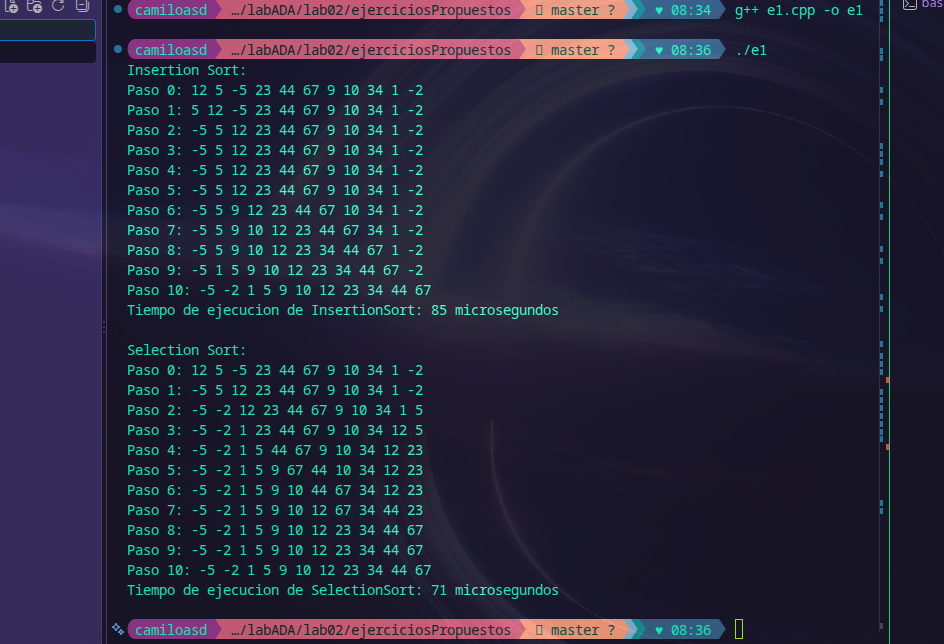
\includegraphics[width=0.8\textwidth]{img/e1.png}
    \caption{Ejecución de e1.cpp}
    \label{fig:diagrama}
    \end{figure}

	\subsection{Ejercicio 2}

        Implementa el algoritmo Insertion Sort para ordenar una lista de $n$ nombres ingresados por el usuario. Analiza su comportamiento con una lista ya ordenada, una lista en orden inverso y una lista aleatoria. ¿Cómo cambia el tiempo de ejecución?
    
    \lstinputlisting[language=c++, caption={Ejercicio 02: InsertionSort en una lista de n nombres y comparaciones con otras listas.},numbers=left,]{../ejerciciosPropuestos/e2.cpp}

    \begin{itemize}
        \item En el código anterior se puede observar el código de la solución alternativa.
        \item De la línea 7 - 21 se implementa la solucion propuesta. 
        \item En la línea 24 - 27 se implementa la solución de Euclides. 
        \item En main() se hace la comparación de ambos algoritmos, dejando en evidencia que Euclides es por mucho más eficiente. 
    \end{itemize}

    \begin{figure}[H]
    \centering
    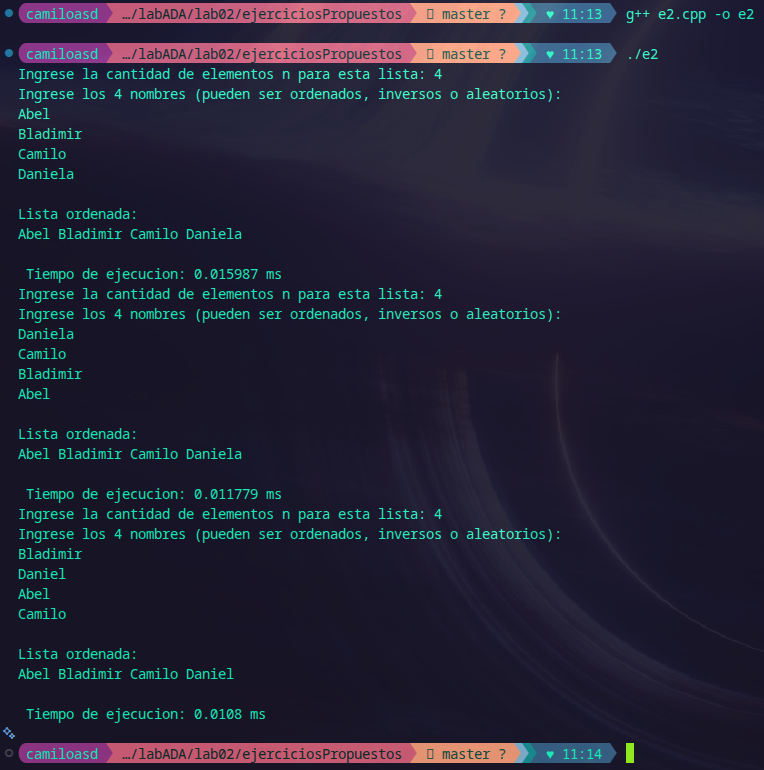
\includegraphics[width=0.9\textwidth]{img/e2.png}
    \caption{Ejecución de e2.cpp}
    \label{fig:diagrama}
    \end{figure}

	\subsection{Ejercicio 3}

		Implementa el algoritmo Selection Sort sobre un arreglo de números flotantes. Muestra el número de comparaciones e intercambios realizados.
    
		\lstinputlisting[language=c++, caption={Ejercicio 03: SelectionSort sobre arreglo de numeros float.},numbers=left,]{../ejerciciosPropuestos/e3.cpp}

    \begin{itemize}
        \item En el código anterior se puede observar el código de la solución alternativa.
        \item De la línea 7 - 21 se implementa la solucion propuesta. 
        \item En la línea 24 - 27 se implementa la solución de Euclides. 
        \item En main() se hace la comparación de ambos algoritmos, dejando en evidencia que Euclides es por mucho más eficiente. 
    \end{itemize}

    \begin{figure}[H]
    \centering
    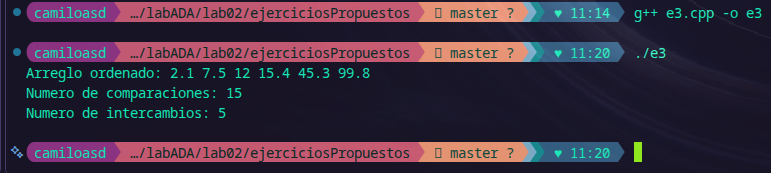
\includegraphics[width=0.8\textwidth]{img/e3.png}
    \caption{Ejecución de e3.cpp}
    \label{fig:diagrama}
    \end{figure}

	\subsection{Ejercicio 4}

		Crea una función que reciba un arreglo y un tipo de ordenamiento (insertion o selection) y aplique el algoritmo correspondiente. Evalúa el rendimiento con 1000, 5000 y 10000 elementos aleatorios.    
		\lstinputlisting[language=c++, caption={Ejercio 04: Función que recibe el tipo de ordenamiento.},numbers=left,]{../ejerciciosPropuestos/e4.cpp}

    \begin{itemize}
        \item En el código anterior se puede observar el código de la solución alternativa.
        \item De la línea 7 - 21 se implementa la solucion propuesta. 
        \item En la línea 24 - 27 se implementa la solución de Euclides. 
        \item En main() se hace la comparación de ambos algoritmos, dejando en evidencia que Euclides es por mucho más eficiente. 
    \end{itemize}

    \begin{figure}[H]
    \centering
    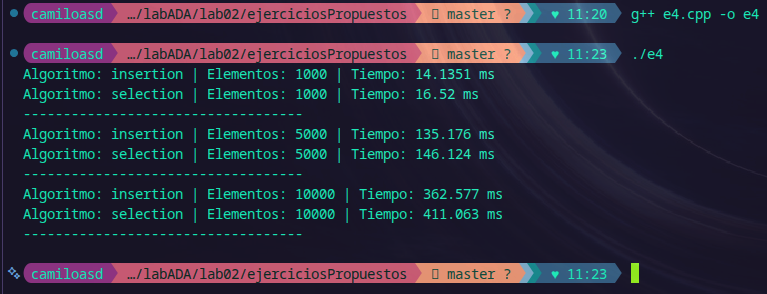
\includegraphics[width=0.8\textwidth]{img/e4.png}
    \caption{Ejecución de e4.cpp}
    \label{fig:diagrama}
    \end{figure}
	
	\subsection{Ejercicio 5}
		Desarrollen una aplicación en C++ que permita ordenar una lista de elementos sobre una temática libre elegida por el estudiante (en este caso, libros). Cada elemento debe contener al menos los siguientes atributos:
		\begin{itemize}
			\item Un identificador o código (string o entero).
			\item Un nombre o título (string).
			\item Un valor numérico que sirva como criterio de ordenamiento (número de páginas).
		\end{itemize}

		\noindent\textbf{Pasos a seguir:}
		\begin{itemize}
			\item Definir la temática y la estructura de los datos.
			\item Cargar los datos dinámicamente desde un archivo \texttt{.txt}.
			\item Ordenar los elementos de mayor a menor según el valor numérico, usando Insertion Sort y Selection Sort.
			\item Implementar contadores para las comparaciones realizadas y los intercambios efectuados.
			\item Medir el tiempo de ejecución.
			\item Exportar la lista ordenada a un archivo \texttt{.csv}.
		\end{itemize}

		\lstinputlisting[language=c++, caption={Ejercio 05: Creación de aplicación que ordena una lista de libros por número de páginas.},numbers=left,]{../ejerciciosPropuestos/e5.cpp}

    \begin{itemize}
        \item En el código anterior se puede observar el código de la solución alternativa.
        \item De la línea 7 - 21 se implementa la solucion propuesta. 
        \item En la línea 24 - 27 se implementa la solución de Euclides. 
        \item En main() se hace la comparación de ambos algoritmos, dejando en evidencia que Euclides es por mucho más eficiente. 
    \end{itemize}

    \begin{figure}[H]
    \centering
    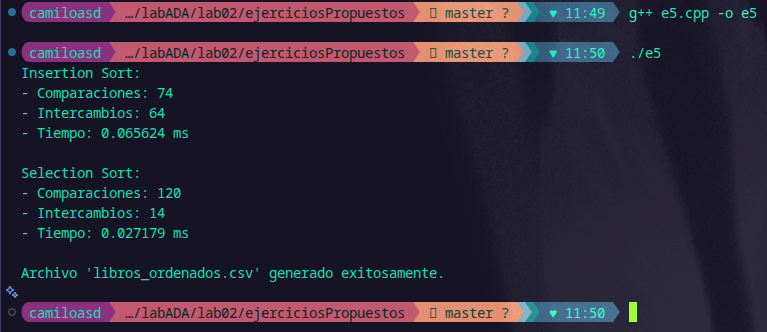
\includegraphics[width=0.95\textwidth]{img/e5(1).png}
    \caption{Ejecución de e5.cpp}
    \label{fig:diagrama}
    \end{figure}

   \begin{figure}[H]
    \centering
    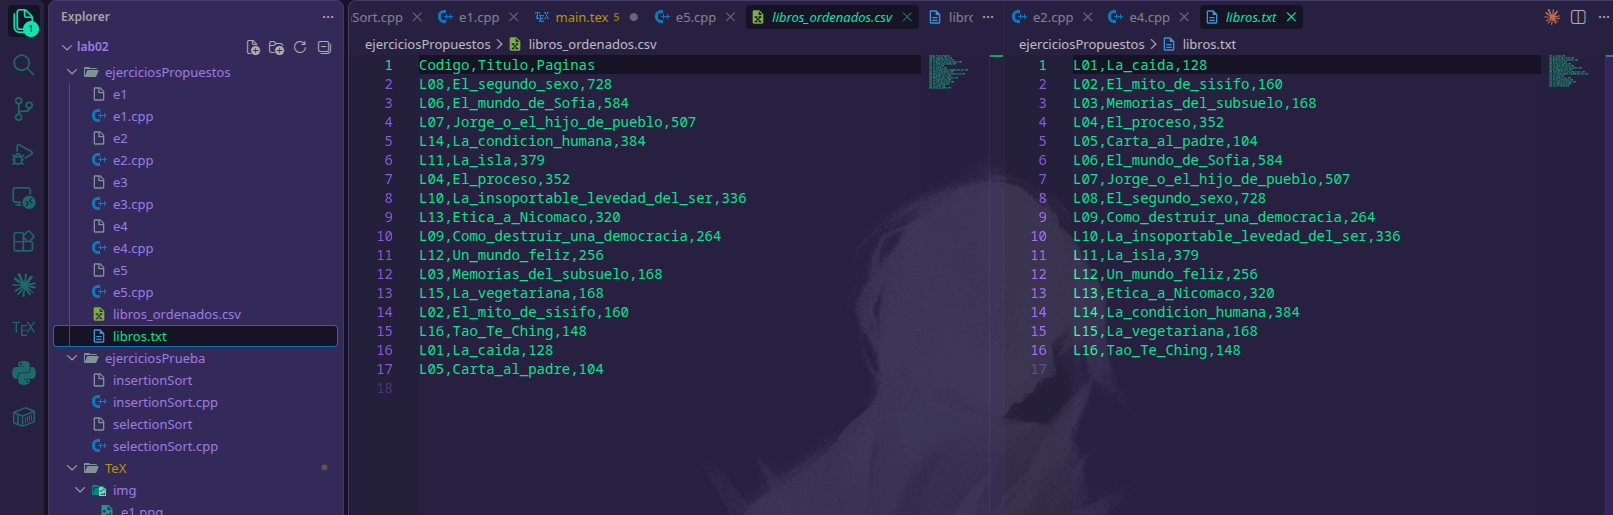
\includegraphics[width=0.95\textwidth]{img/e5(2).png}
    \caption{Comparacion de .csv (ordenado por n° de páginas) vs .txt (desordenado por n° de páginas)}
    \label{fig:diagrama}
    \end{figure}


	\section{Cuestionario}
		\begin{enumerate}
			\item Explica con tus propias palabras: ¿cuál de los dos algoritmos es más eficiente si la lista ya está ordenada? ¿Por qué? Usa un ejemplo distinto al visto en clase.
			\item En tus palabras, ¿qué significa que un algoritmo sea ``in-place''? Da un ejemplo de tu vida cotidiana donde ``ordenar sin usar espacio extra'' tendría sentido.
			\item ¿Por qué se dice que Selection Sort no es estable? Describe un caso concreto (puede ser inventado por ti) donde eso cause un problema real.
			\item ¿Qué parte te costó más entender entre Insertion Sort y Selection Sort, y cómo la resolviste?
			\item Si tuvieras que explicarle a un compañero que faltó a la práctica cómo optimizar uno de estos dos algoritmos, ¿qué le dirías?
		\end{enumerate}

	\section{Conclusiones}

	%\begin{itemize}	
	%	\item Se creo el archivo \textbf{.gitignore} para no considerar los archivos %\textbf{*.class} que son innecesarios hacer seguimiento.
	%\end{itemize}
	%\begin{lstlisting}[language=bash,caption={Creando .gitignore}]
	%	$ vim lab01/.gitignore
	%\end{lstlisting}
	%\begin{lstlisting}[language=bash,caption={lab01/.gitignore}]
	%	*.class
	%\end{lstlisting}
	%\begin{lstlisting}[language=bash,caption={Commit: Creando .gitignore para archivos *.class}]
	%	$ git add .
	%	$ git commit -m "Creando .gitignore para archivos *.class"			
	%	$ git push -u origin main
	%\end{lstlisting}
	
	%\begin{lstlisting}[language=bash,caption={Creando .gitignore}]
	%	$ vim lab01/Insertion.java
	%\end{lstlisting}
	
    
\section{Referencias}
\begin{itemize}
    \item Wikipedia. (2025). \textit{Máximo común divisor}. Recuperado de \url{https://es.wikipedia.org/wiki/M\%C3\%A1ximo_com\%C3\%BAn_divisor}
    \item Wikipedia. (2025). \textit{Algoritmo de Euclides}. Recuperado de \url{https://es.wikipedia.org/wiki/Algoritmo_de_Euclides}
    \item Informatec Digital. (2025). \textit{El Algoritmo de Euclides: Historia, Uso y Aplicaciones}. Recuperado de \url{https://informatecdigital.com/el-algoritmo-de-euclides/}
\end{itemize}
	
%\clearpage
%\bibliographystyle{apalike}
%\bibliographystyle{IEEEtranN}
%\bibliography{bibliography}
			
\end{document}\noindent\textbf{Enunciado:} 